Phân tích khám phá giúp hiểu rõ cấu trúc dữ liệu, nhận diện các đặc điểm của giao dịch gian lận và phát hiện giá trị bất thường trước khi xây dựng mô hình. Quá trình này sử dụng các thư viện \texttt{seaborn} và \texttt{matplotlib} để trực quan hóa kết quả.

\section{Phân bố dữ liệu}
Hình \ref{fig:distributions} mô tả phân bố của ba đặc trưng số chính: logarit số tiền giao dịch \texttt{amt\_log}, tần suất giao dịch \texttt{txn\_freq\_hour} và khoảng cách \texttt{distance\_km}. Cả ba biến đều phân bố lệch về bên trái: phần lớn giao dịch có số tiền nhỏ, mỗi thẻ chỉ giao dịch một vài lần trong một giờ và khoảng cách từ đơn vị chấp nhận thanh toán đến vị trí thường trú của thẻ thường không quá 150 km. Phần đuôi dài bên phải của phân bố chứa các giá trị bất thường, nơi tập trung nhiều giao dịch gian lận.

\begin{figure}[H]
    \centering
    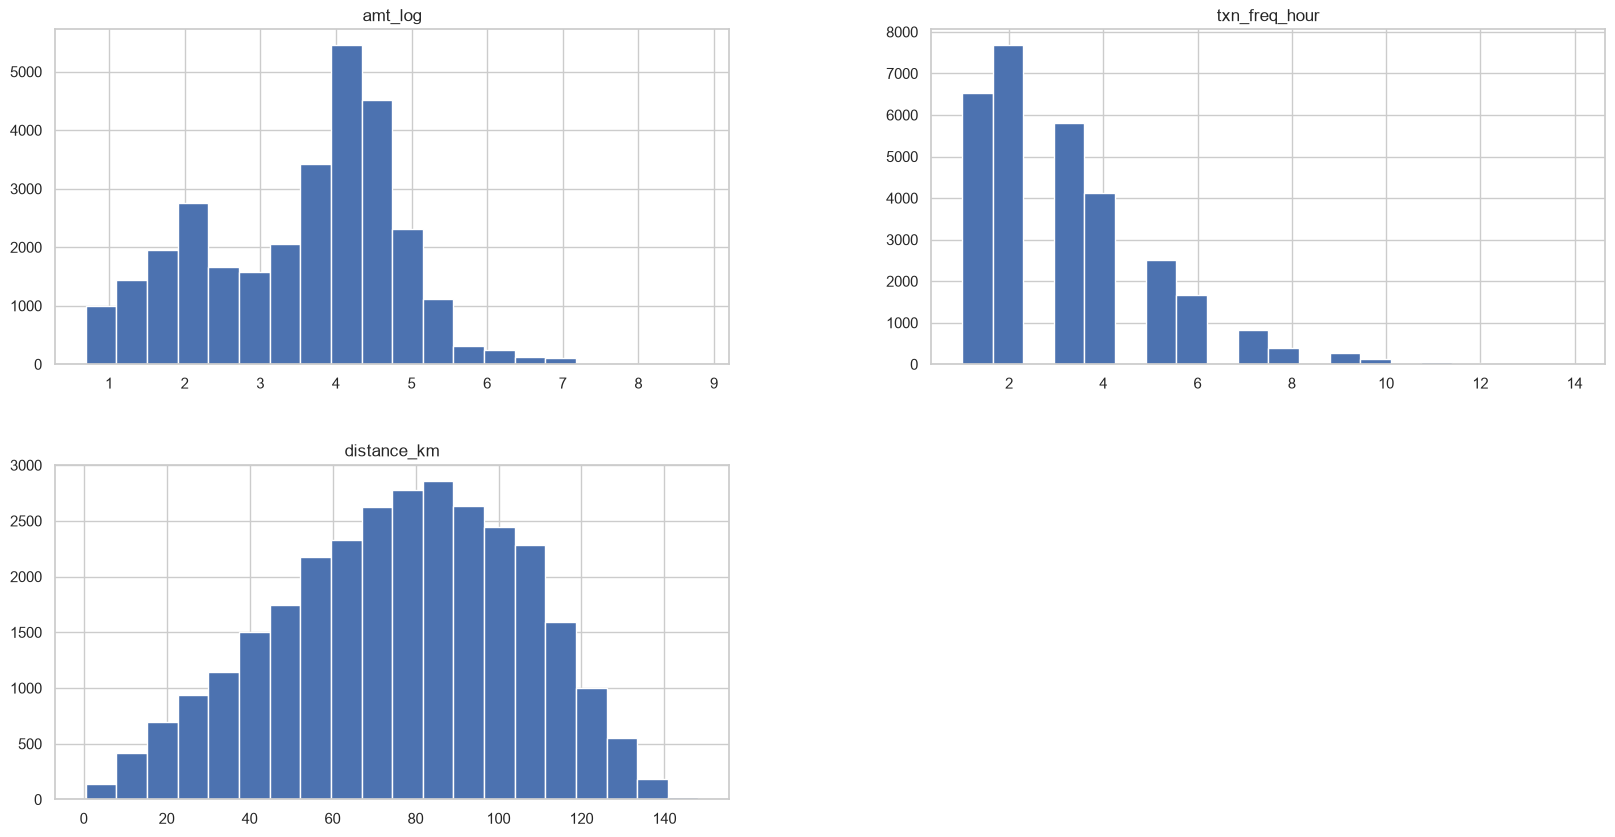
\includegraphics[width=1.0\linewidth]{figures/fig_distributions.png}
    \caption{Phân bố của các đặc trưng số trong bộ dữ liệu}
    \label{fig:distributions}
\end{figure}

\section{Gian lận theo loại hình dịch vụ}
Hình \ref{fig:fraud_category} thể hiện tỷ lệ gian lận của 10 loại hình dịch vụ có rủi ro cao nhất. Ba nhóm đầu là \texttt{shopping\_net}, \texttt{misc\_net} và \texttt{grocery\_pos} chiếm 82 trong tổng số 133 vụ gian lận, tương ứng 61{,}7\%. Loại \texttt{shopping\_net} có tỷ lệ gian lận cao nhất với 33 trong 2\,302 giao dịch, tương ứng 1{,}43\%, trong khi nhóm an toàn nhất \texttt{personal\_care} chỉ có 4 trong 2\,220 giao dịch, tương ứng 0{,}18\%. Kết quả kiểm định Chi-square cho giá trị $p = 1{,}28 \times 10^{-23}$, khẳng định loại hình dịch vụ có liên quan có ý nghĩa thống kê với gian lận, do đó \texttt{category} được giữ lại làm đặc trưng cho mô hình.

\begin{figure}[H]
    \centering
    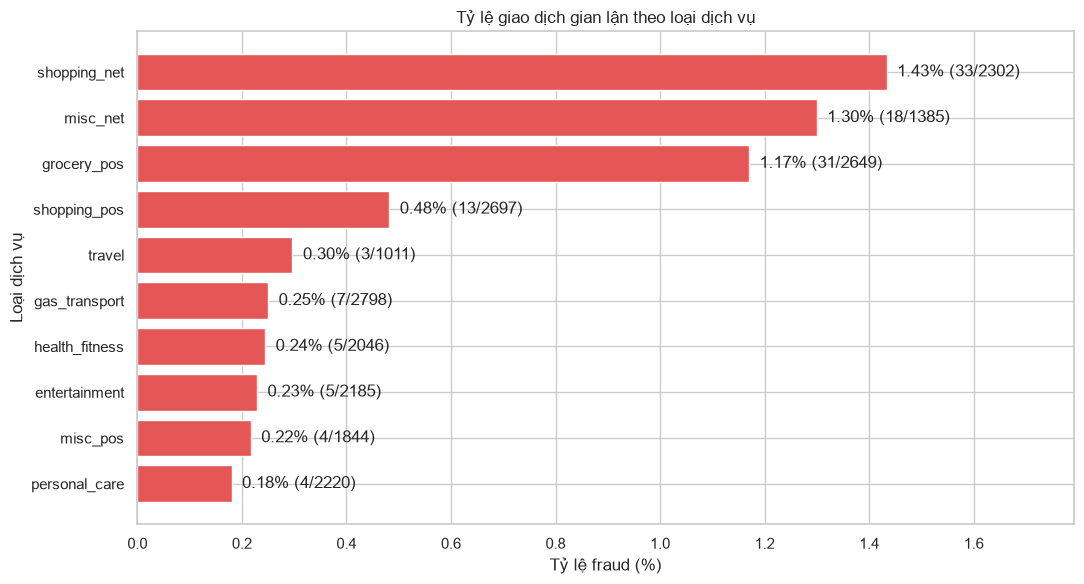
\includegraphics[width=0.9\linewidth]{figures/fig_fraud_category.png}
    \caption{Tỷ lệ giao dịch gian lận theo loại hình dịch vụ}
    \label{fig:fraud_category}
\end{figure}

\section{Giá trị bất thường}
Hình \ref{fig:outlier} dùng biểu đồ hộp để khảo sát giá trị bất thường của các đặc trưng số, và Bảng \ref{tab:outlier} thống kê chi tiết theo quy tắc $1{,}5 \times \text{IQR}$.

\begin{figure}[H]
    \centering
    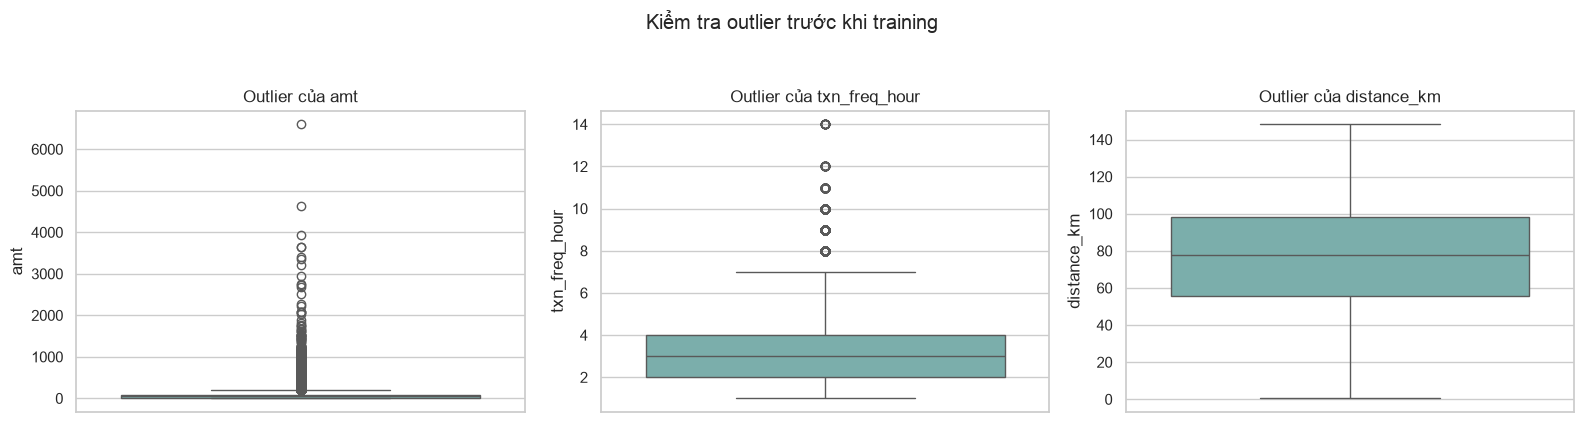
\includegraphics[width=1.0\linewidth]{figures/fig_outliers.png}
    \caption{Biểu đồ hộp kiểm tra giá trị bất thường}
    \label{fig:outlier}
\end{figure}

\begin{table}[H]
\centering
\fontsize{11}{13.6}\selectfont
\renewcommand{\arraystretch}{1.2}
\setlength{\tabcolsep}{6pt}
\begin{tabularx}{\textwidth}{|p{3.4cm}|p{2.5cm}|p{2.5cm}|X|}
\hline
\textbf{Đặc trưng} & \textbf{Ngưỡng trên} & \textbf{Số giá trị bất thường (tỷ lệ)} & \textbf{Gian lận trong vùng bất thường} \\
\hline
amt & 192{,}16 & 1\,521 (5{,}06\%) & 104 (78{,}2\%) \\
\hline
txn\_freq\_hour & 7{,}00 & 887 (2{,}95\%) & 5 \\
\hline
distance\_km & 162{,}10 & 0 (0\%) & 0 \\
\hline
\end{tabularx}
\caption{Thống kê giá trị bất thường theo quy tắc IQR}
\label{tab:outlier}
\end{table}

Đáng chú ý, 78{,}2\% số giao dịch gian lận nằm trong vùng giá trị bất thường của cột \texttt{amt}. Vì vậy, đồ án không xóa bỏ các giá trị bất thường ngay ở bước này mà chỉ giới hạn chúng theo quy tắc IQR sau khi chia tập huấn luyện và tập kiểm tra, nhằm tránh làm mất đi chính những giao dịch gian lận.



\section{Quan hệ giữa các đặc trưng}

\begin{figure}[H]
	\centering
	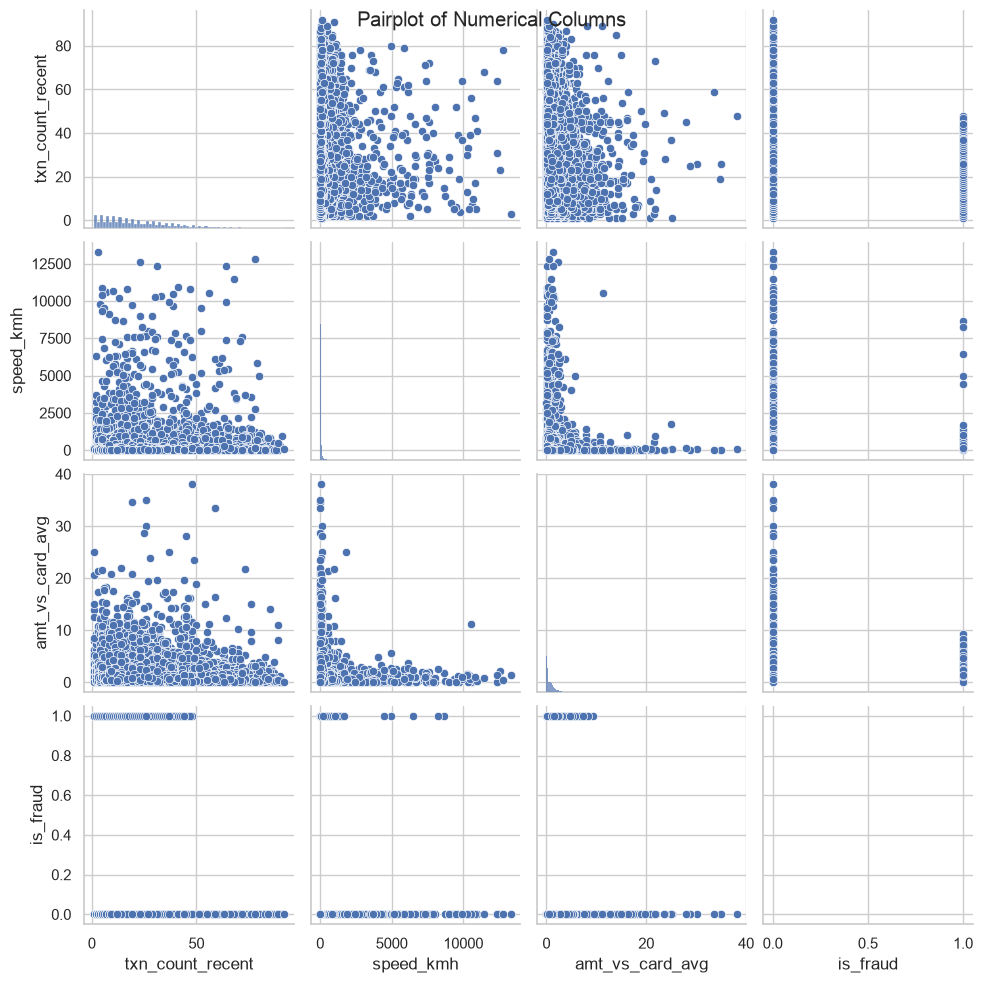
\includegraphics[width=0.9\linewidth]{figures/fig_scatter_features.png}
	\caption{Quan hệ cặp giữa các đặc trưng hành vi theo nhãn gian lận}
	\label{fig:scatter_features}
\end{figure}

Hình \ref{fig:scatter_features} trình bày quan hệ cặp giữa ba đặc trưng hành vi gồm số lần giao dịch gần đây \texttt{txn\_count\_recent}, tốc độ di chuyển \texttt{speed\_kmh} và tỷ lệ số tiền so với trung bình thẻ \texttt{amt\_vs\_card\_avg}, tô màu theo nhãn gian lận. Giao dịch gian lận có tốc độ di chuyển và tỷ lệ số tiền so với trung bình thẻ cao hơn rõ rệt: trung vị \texttt{speed\_kmh} là 59{,}4 km/h so với 21{,}2 km/h của giao dịch hợp lệ, trung vị \texttt{amt\_vs\_card\_avg} là 1{,}94 so với 0{,}67, cho thấy gian lận thường phát sinh ở nơi xa nơi ở quen thuộc và với số tiền vượt trung bình chi tiêu của thẻ. Ngược lại, \texttt{txn\_count\_recent} gần như không phân biệt hai lớp (trung vị 20 so với 19), nên chủ yếu đóng vai trò đặc trưng bổ trợ.



Qua các phân tích trên, 14 đặc trưng được chọn để đưa vào mô hình gồm: \texttt{amt}, \texttt{age}, \texttt{amt\_vs\_card\_median}, \texttt{hour}, \texttt{txn\_freq\_hour}, \texttt{distance\_km}, \texttt{category}, \texttt{amt\_log}, \texttt{amt\_zscore\_card}, \texttt{is\_night}, \texttt{speed\_kmh}, \texttt{amt\_per\_km}, \texttt{txn\_count\_recent} và \texttt{amt\_vs\_card\_avg}. Các cột định danh như \texttt{cc\_num} hay \texttt{trans\_num} không được dùng trực tiếp vì mô hình có thể học thuộc mã thay vì học quy luật tổng quát của gian lận.